%%%%%%%%%%% Implementation Details %%%%%%%%%%%%%%%%%
\chapter{Implementation Details} \label{ch4_implementation}
\markboth{Implementation Details}{Implementation Details}

This chapter details the technical implementation of the architectural design proposed for the blockchain system described in the previous chapter. It provides a comprehensive walkthrough of the implementation methodologies, focusing on the modular Python core-blockchain backend and the blockchain explorer frontend implementation using Vue.js for visualization.
The full source code for this implementation is open-source and available on GitHub to facilitate student experimentation from this link:\url{https://github.com/Mostamhd/blockchain-educational-system}

\section{Development Environment and Technology Stack} \label{ch4_tech_stack}

The system relies on a containerized microservices architecture to ensure consistent behavior across different educational environments (e.g., student laptops vs. university lab servers). The core technologies selected for this implementation include:

\begin{itemize}
    \item \textbf{Language:} Python 3.9 was selected for the backend due to its extensive support for cryptographic libraries and high readability, which facilitates the "glass-box" educational approach \cite{python_lang}.
    \item \textbf{API Framework:} \textit{FastAPI} (wrapped via Uvicorn) is utilized to expose the blockchain's functionality via RESTful endpoints, allowing the communication between the backend node and the frontend client.
    \item \textbf{Cryptography:} The system utilizes the \textit{eth-keys} and \textit{eth-utils} libraries. This makes the project matches with Ethereum's cryptographic standards, employing \textbf{Keccak-256} for hashing and \textbf{ECDSA} (SECP256k1) for digital signatures, providing students with exposure to a production like Ethereum primitives \cite{wood2014ethereum}.
    \item \textbf{Frontend:} \textit{Vue.js} which is used to power the Blockchain Explorer, providing a user interface that visualizes block propagation, validators, and mempool status in real-time \cite{vuejs}.
    \item \textbf{Containerization:} \textit{Docker} and \textit{Docker Compose} are used to orchestrate the multi-node network, allowing students and teachers to simulate a distributed consensus network on a single physical machine \cite{docker}.
\end{itemize}

\section{Core Blockchain Architecture} \label{ch4_core_architecture}

The blockchain system implementation is structured around several key classes that manage the distributed ledger's state.

\subsection{The Account Model} \label{ch4_account_model}
In this system, unlike in Bitcoin, which uses an Unspent Transaction Output (UTXO) model, this system implements an \textbf{Account-based Model} (similar to Ethereum). This design choice was made to simplify the state logic for students, making it easier to track balances and understand global state transitions.

The \texttt{AccountModel} class (\texttt{blockchain/transaction/account\_model.py}) maintains the global state of user balances. \textbf{Data Persistence Note:}
For the purpose of this educational prototype, the state is maintained in volatile memory (Python dictionaries). This allows for rapid iteration and modification during laboratory exercises. In a production-grade application, this in-memory structure would be replaced by a persistent key-value store (such as LevelDB) or an authenticated data structure like a Merkle Patricia Trie. This would ensure data durability and provide cryptographically verifiable state roots, as detailed in the Ethereum Yellow Paper \cite{wood2014ethereum}.

\newpage
\begin{lstlisting}[language=Python, caption=Account Model Implementation, label=lst:account_model]
class AccountModel:
    def __init__(self):
        self.accounts = []
        self.balances = {}

    def update_balance(self, public_key_string, amount):
        if public_key_string not in self.accounts:
            self.add_account(public_key_string)
        self.balances[public_key_string] += amount
\end{lstlisting}

\subsection{Transaction Management} \label{ch4_transaction_impl}
A transaction is the atomic unit that represents a change in the state of a blockchain. In the blockchain system implemented,

the \texttt{Transaction} class (\texttt{blockchain/transaction/transaction.py}) encapsulates the transfer logic. It supports different types of transaction payloads, such as \texttt{TRANSFER} for currency ,\texttt{EXCHANGE} for system operations, and \texttt{COINBASE} for the block reward used in the consensus mechanism. 

Crucially, every transaction includes a unique id hash calculated based on the transaction payload, as seen in the \texttt{payload} method. Additionally, every transaction includes a timestamp to prevent replay attacks. The \texttt{sign} method ensures non-repudiation using the sender's private key.

\begin{lstlisting}[language=Python, caption=Transaction Structure, label=lst:transaction_class]
class Transaction:
    def __init__(self, sender_public_key, receiver_public_key, amount, type):
        self.sender_public_key = sender_public_key
        self.receiver_public_key = receiver_public_key
        self.amount = amount
        self.type = type
        self.id = uuid.uuid1().hex
        self.timestamp = time.time()
        self.signature = ""

    def sign(self, signature: str) -> None:
        if not isinstance(signature, str):
            raise TypeError("Signature must be a string")
        self.signature = signature

    def payload(self):
        json_representation = copy.deepcopy(self.to_dict())
        json_representation['signature'] = ''
        return json_representation
\end{lstlisting}

\subsection{The Transaction Pool (Mempool)}
Before transactions are included in a block, they reside in the \texttt{TransactionPool}. This class acts as a holding buffer for pending operations. In a distributed asynchronous network, transactions arrive at different times, awaiting execution. The TransactionPool, also known as the mempool, ensures that nodes can temporarily store valid transactions that have been broadcast but not yet confirmed and are currently awaiting execution.

The implementation includes logic to prevent double-spending and duplication. Before adding a transaction, the pool checks if the transaction `id` already exists or if the signature is invalid. This ensures that the transaction provided to the next block creator is clean and valid.

\section{The Network Node} \label{ch4_node_impl}

The \texttt{Node} class (\texttt{blockchain/node/node.py}) acts as the central orchestrator of the system. as the node class integrates three critical subsystems of the blockchain:
\begin{enumerate}
    \item \textbf{The P2P Layer:} For communicating between the nodes in the blockchain network.
    \item \textbf{The Blockchain Core:} For maintaining the ledger state and consensus.
    \item \textbf{The REST API:} For external interaction with the node itself (like a Wallet application or Explorer).
\end{enumerate}

\newpage

\subsection{Concurrency and Threading}
To maintain responsiveness, the node utilizes Python's \texttt{threading} module. Since the P2P listener and the API server are blocking operations, they must run in parallel to the block production loop.

\begin{lstlisting}[language=Python, caption=Node Initialization and Threading, label=lst:node_init]
class Node:
    def __init__(self, ip, port, api_port, key=None):
        self.transaction_pool = TransactionPool()
        self.wallet = Wallet()
        self.blockchain = Blockchain()
        
        self.start_p2p()
        self.start_node_api()
        self.start_produce_block()

    def run_produce_block(self):
        while self.keep_running:
            self.produce_block()
            time.sleep(10) # Block time
\end{lstlisting}

\subsection{Consensus and Blocks Forging Logic}
The node implements the Proof of Stake consensus logic, which functions as the deterministic lottery explained earlier in the thesis. The \texttt{produce\_block} method is the core part of creating or forging a block. It queries the consensus module to calculate the \texttt{next\_forger} based on the hash of the previous block and the current stake distribution.

If the local node's public key matches the calculated forger, the node proceeds to:
\begin{enumerate}
    \item Bundle pending transactions from the Transaction pool.
    \item Execute the transactions to verify state changes.
    \item Cryptographically seal the block with a signature.
    \item Broadcast the new block to all connected peers via the P2P layer.
\end{enumerate}

\begin{lstlisting}[language=Python, caption=Block Production Logic, label=lst:produce_block]
def produce_block(self):
    forger = self.blockchain.next_forger()
    
    if forger == self.wallet.public_key_string():
        # Create the block
        block = self.blockchain.create_block(
            self.transaction_pool.transactions, 
            self.wallet
        )
        message = Message(self.p2p.socket_connector, 'BLOCK', block)
        self.p2p.broadcast(BlockchainUtils.encode(message))
\end{lstlisting}

\section{Visualization Layer (Blockchain Explorer)} \label{ch4_explorer}

For the second component of the blockchain system, the \textbf{Blockchain Explorer} was developed to help users visualize the data in the blockchain. The \textbf{Blockchain Explorer} was developed using \textbf{Vue.js}. This frontend application connects to the Python node's REST API to provide a more user-friendly way to view the network's internal state.

The explorer is divided into several functional views, as illustrated in the following figures.

\newpage

\subsection{Network Dashboard}
The main dashboard (Figure \ref{fig:explorer_dashboard}) provides a high-level overview of the blockchain, displaying the current block height, the transaction pool status, and the list of connected peers.

\begin{figure}[H]
    \centering
    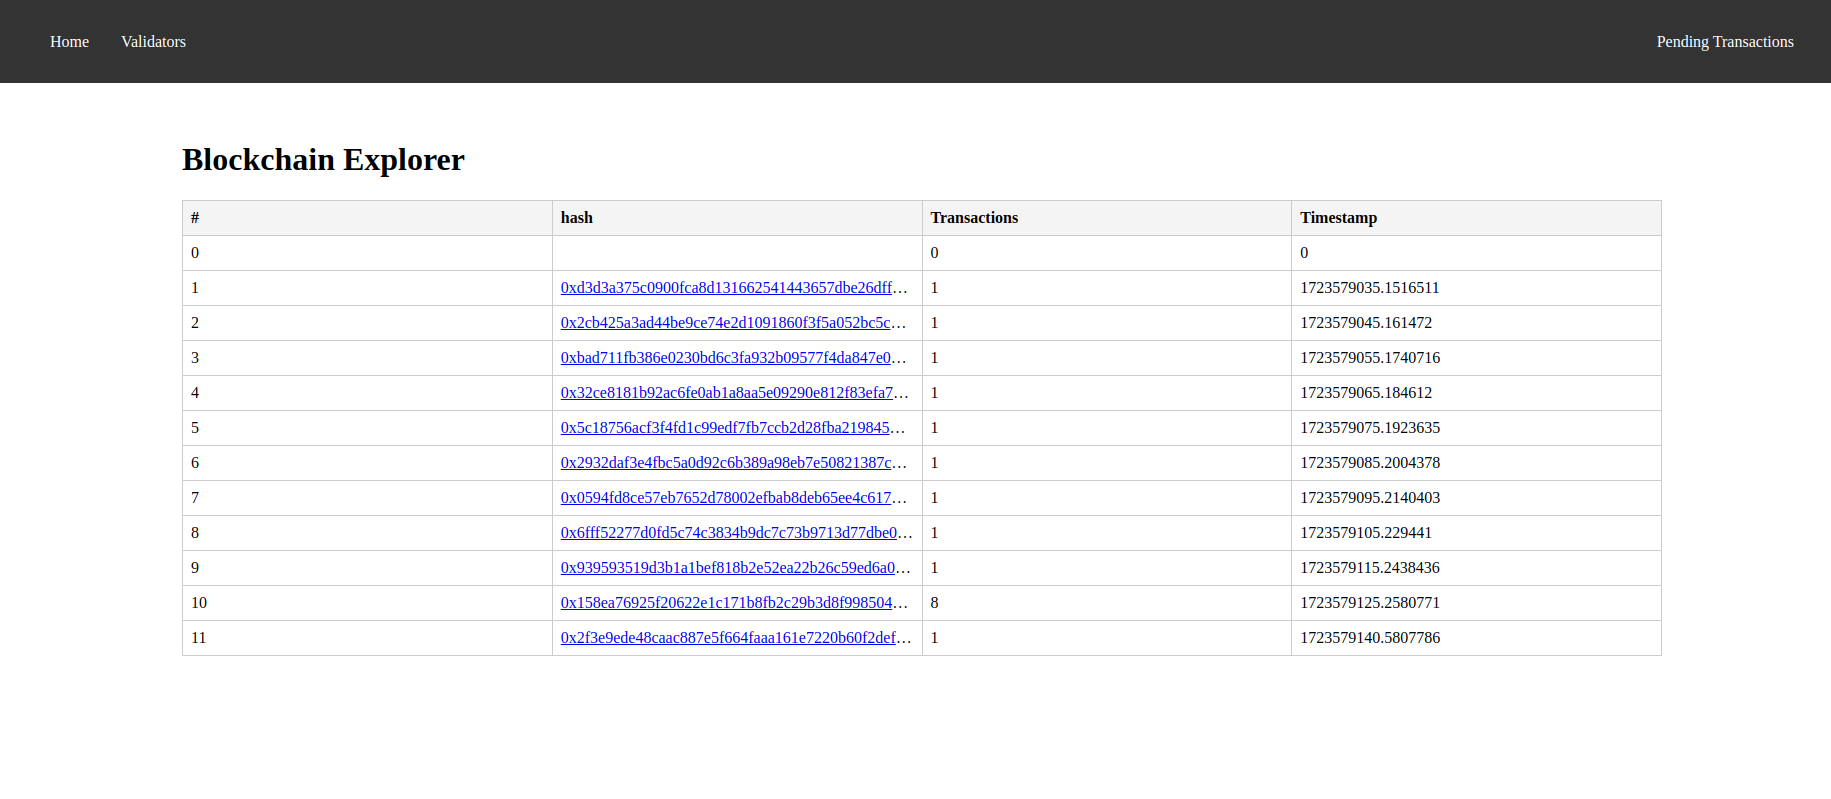
\includegraphics[width=1\textwidth]{figures/explorer_dashboard.png}
    \caption{The Blockchain Explorer Dashboard showing real-time network statistics.}
    \label{fig:explorer_dashboard}
\end{figure}

\subsection{Block Inspection}
Students can click on any block to inspect its details (Figure \ref{fig:explorer_block_details}). This view visualizes the cryptographic link between blocks (Previous Hash) and lists the transactions included in that block.

\begin{figure}[H]
    \centering
    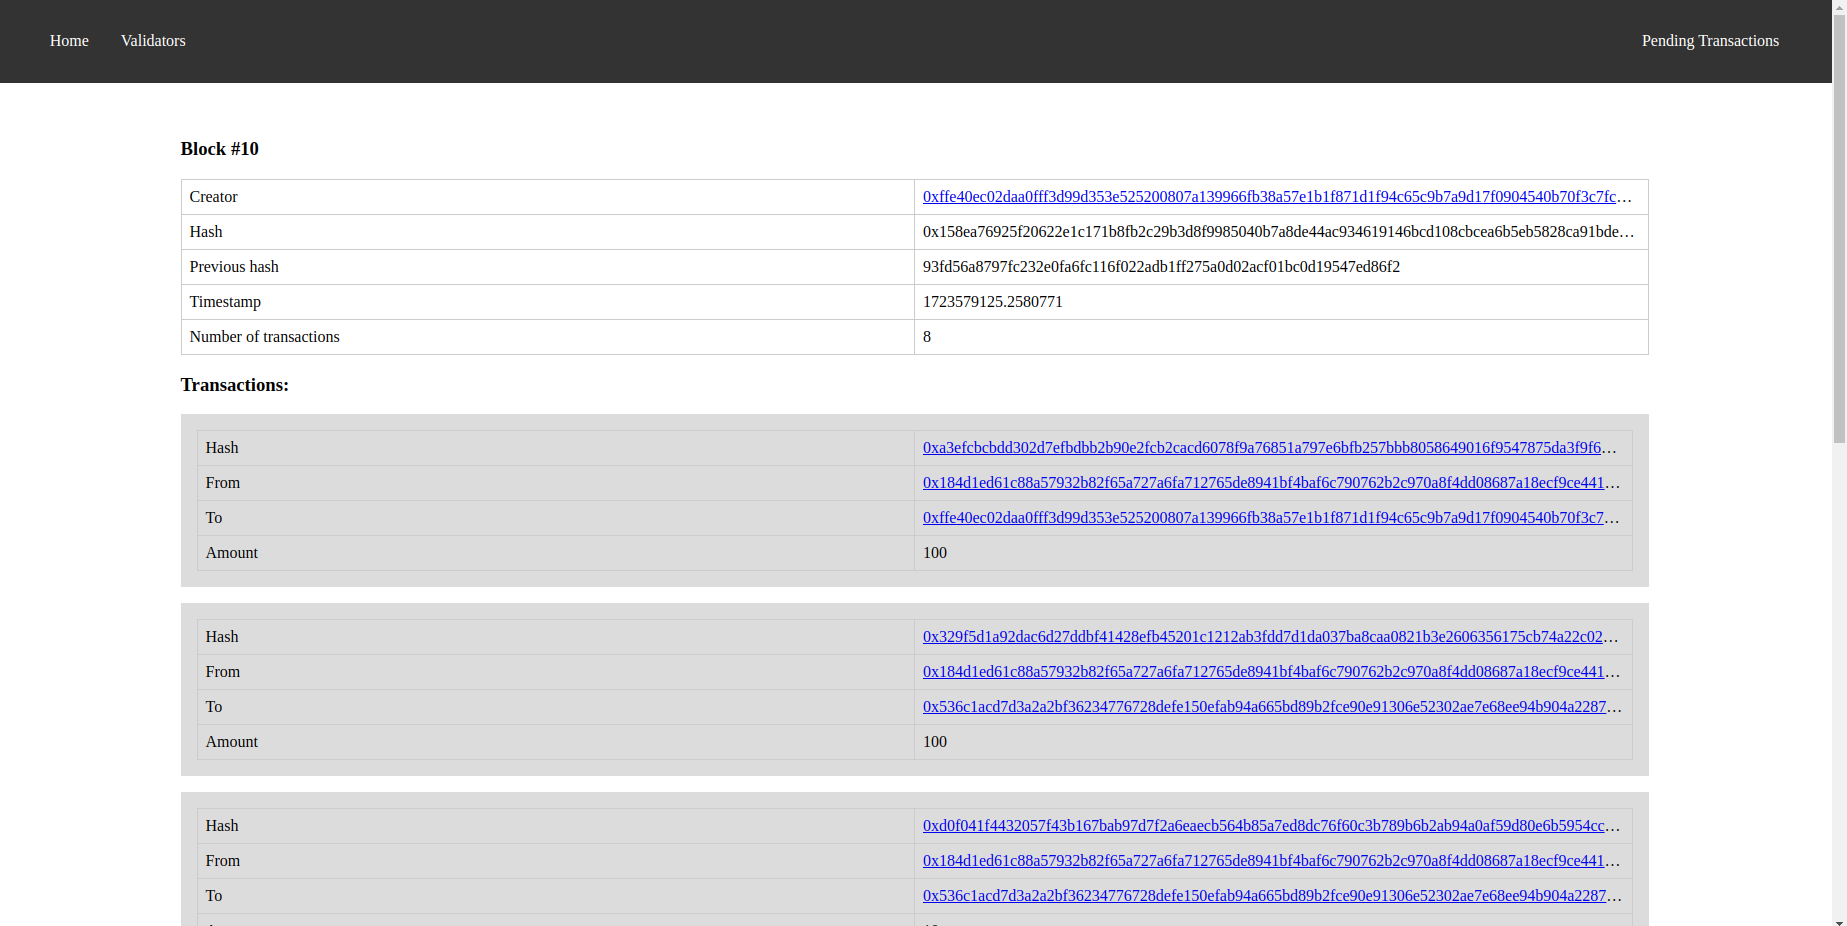
\includegraphics[width=0.9\textwidth]{figures/explorer_block_details.png}
    \caption{Detailed view of a mined block, showing the Forger and Transaction list.}
    \label{fig:explorer_block_details}
\end{figure}

\subsection{Transaction Inspection}
When a student clicks on a transaction hash in the interface, they are navigated to the Transaction Details view (Figure \ref{fig:explorer_transaction_details}). This page is critical for understanding the anatomy of a transaction and how it changes the state of the blockchain.

It breaks down a transaction into its different parts:
\begin{itemize}
    \item \textbf{Metadata:} The unique Transaction ID and the Timestamp.
    \item \textbf{Transfer Logic:} The Sender and Receiver public keys, along with the transferred Amount.
    \item \textbf{Cryptographic Proof:} The ECDSA Signature generated by the sender's private key.
\end{itemize}

This view allows students to visually verify the transaction data and structure matches the \texttt{Transaction} class definition in the backend code.

\begin{figure}[H]
    \centering
    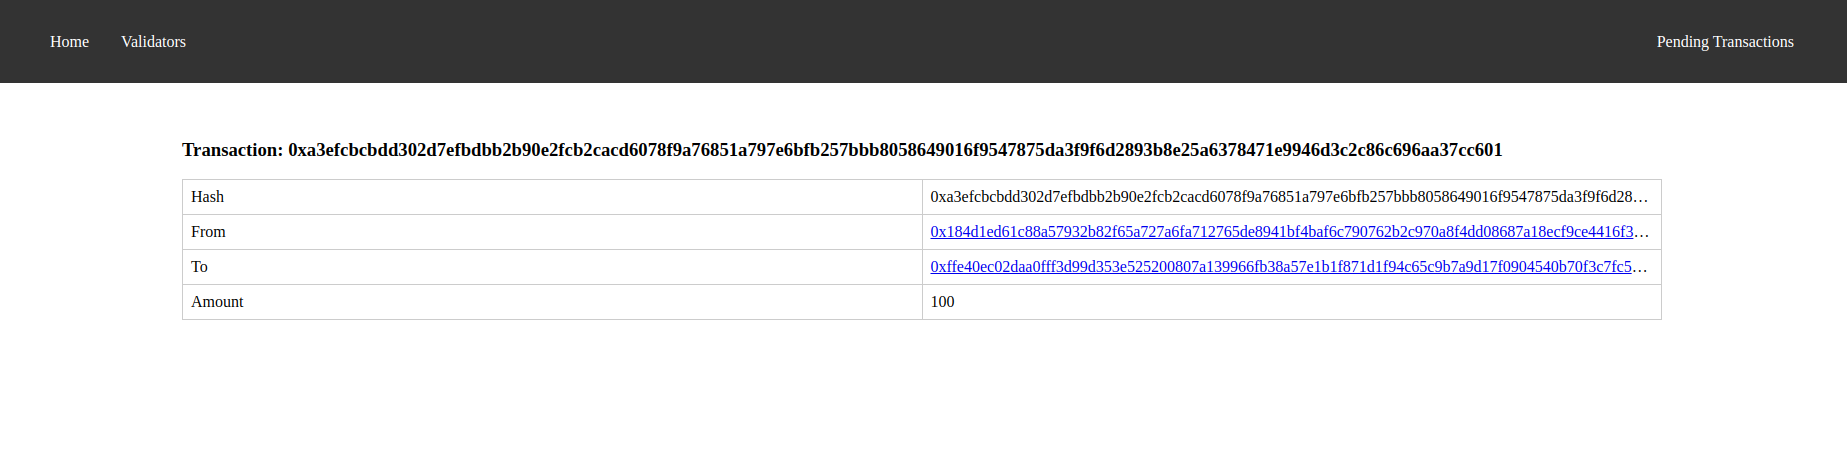
\includegraphics[width=0.9\textwidth]{figures/explorer_trasaction_details.png}
    \caption{Detailed view of a single transaction, exposing the cryptographic signature and transfer amounts.}
    \label{fig:explorer_transaction_details}
\end{figure}

\subsection{Address and Balance Monitoring}
The Address Details view shown (Figure \ref{fig:explorer_address_details}) acts as a personal ledger for a specific blockchain network address. By querying the \texttt{AccountModel} endpoint, this page displays:
\begin{enumerate}
    \item \textbf{Current Balance:} The aggregate result of all historical state changes for the account balance calculated by the node.
    \item \textbf{Transaction History:} A chronological list of all transactions where the address is either involved as a sender or as a receiver.
\end{enumerate}

This component is particularly useful during the "Library Management" module (Chapter 5), as it allows students to track the "Book Token" inventory of the library account versus the student accounts.

\begin{figure}[H]
    \centering
    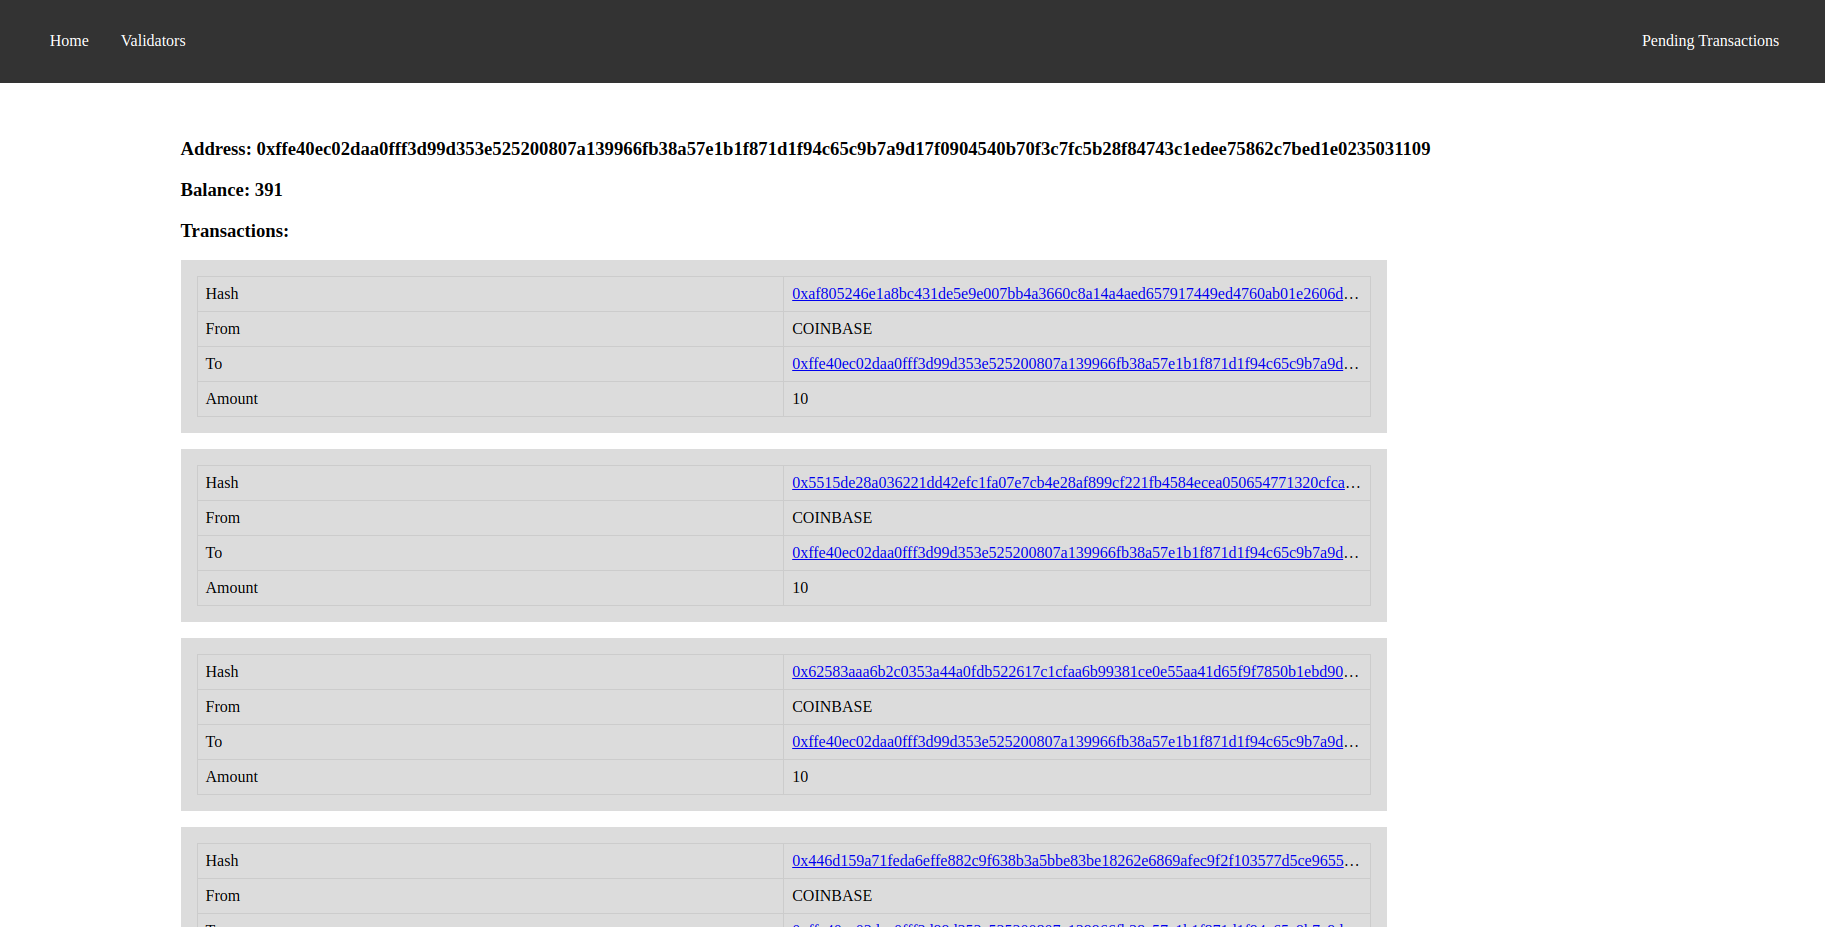
\includegraphics[width=0.9\textwidth]{figures/explorer_address_details.png}
    \caption{The Address Details view showing the current balance and transaction history for a specific wallet.}
    \label{fig:explorer_address_details}
\end{figure}

\subsection{Mempool Visualization}
To understand transaction propagation, the Mempool view (Figure \ref{fig:explorer_mempool}) shows transactions that have been broadcast but not yet confirmed. This helps students visualize network latency and the concept of "pending state."

\begin{figure}[H]
    \centering
    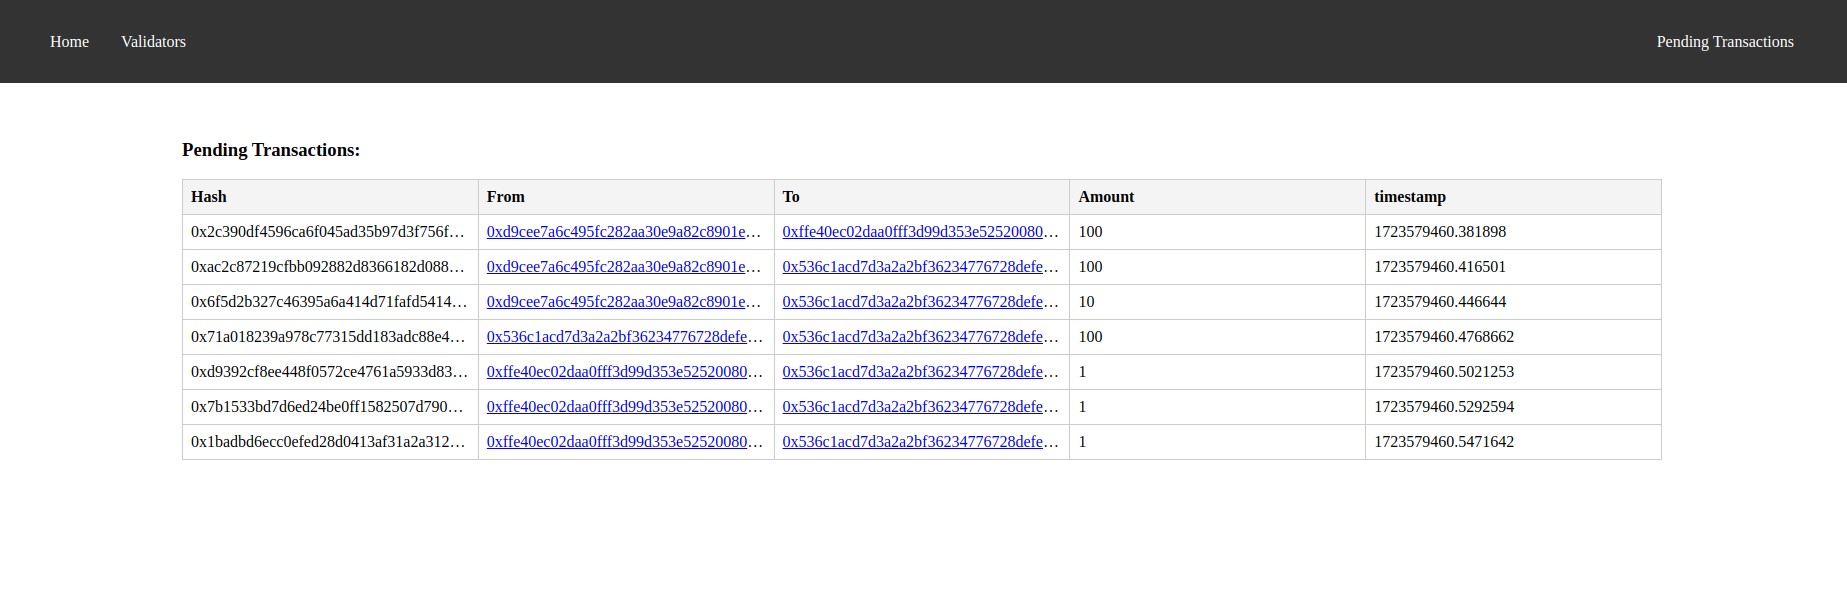
\includegraphics[width=0.9\textwidth]{figures/explorer_mempool.png}
    \caption{The Mempool view displaying pending transactions waiting for confirmation.}
    \label{fig:explorer_mempool}
\end{figure}

\newpage
\subsection{Validator Inspection}
The Validators view shown in (Figure \ref{fig:explorer_validators}) provides a real-time list of the current staker nodes participating in the consensus of the network, as in a Proof of Stake system, transparency regarding network participants is essential for the trust in the network security.

This view queries the blockchain system to display:
\begin{itemize}
    \item \textbf{Name:} The name of the validator provided to the network.
    \item \textbf{IP:} The IP address the validator client is running from.
    \item \textbf{Port:} The Port the validator client is running on.
\end{itemize}

\begin{figure}[H]
    \centering
    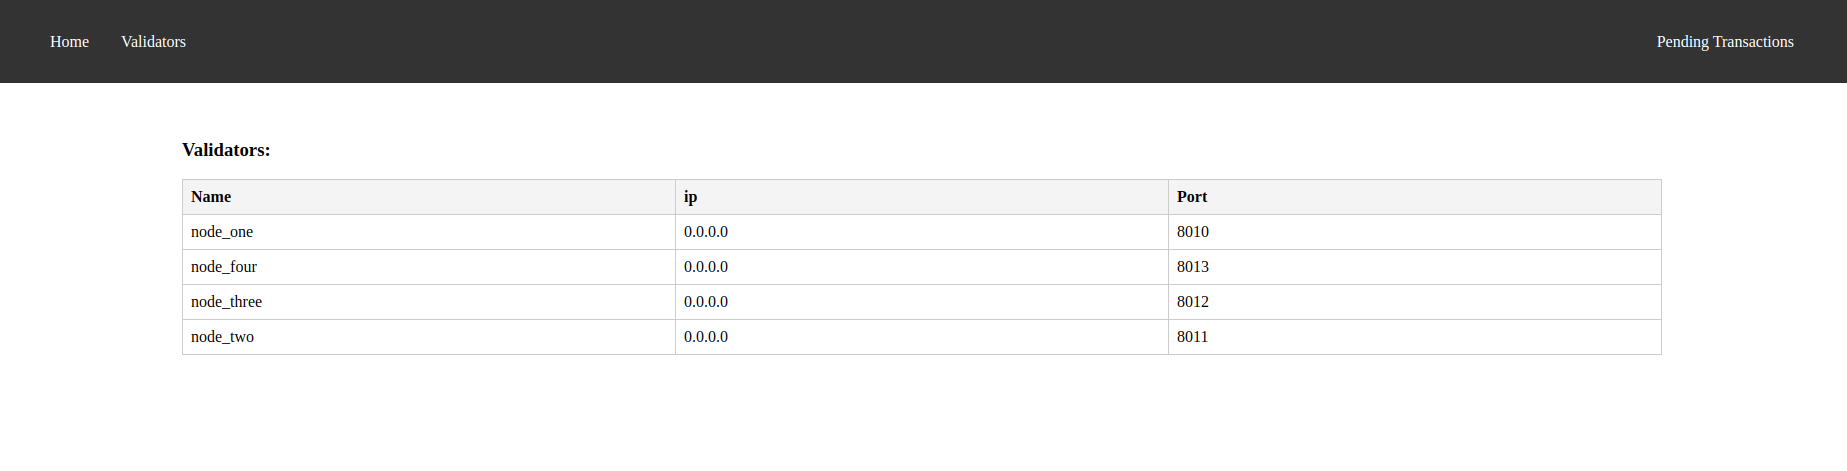
\includegraphics[width=0.9\textwidth]{figures/explorer_validators_details.png}
    \caption{The Validators dashboard showing active stakers and their respective validation weights.}
    \label{fig:explorer_validators}
\end{figure}
\section{Testing and Validation} \label{ch4_testing}

% To ensure the reliability of the system for educational use, a unit testing suite was implemented using Python's \texttt{unittest} framework. The tests focus on the integrity of the cryptographic primitives and the consensus logic.



% Key validation areas include:
% \begin{itemize}
%     \item \textbf{Hashing Determinism:} Verifying that the \texttt{BlockchainUtils.hash()} method (utilizing Keccak-256) produces consistent outputs for identical inputs.
%     \item \textbf{Chain Continuity:} Automated tests ensure that any tampering with historical block data causes the \texttt{is\_chain\_valid()} check to fail.
%     \item \textbf{Signature Verification:} Validating that transactions signed with an incorrect private key are rejected by the \texttt{Wallet.signature\_valid()} method.
% \end{itemize}

% This robust testing infrastructure ensures that students are working with a stable core system before they attempt the modifications described in the Curriculum Design chapter.
\section{Summary}
This chapter presented the technical implementation of the \textit{Blockchain System}. We created a modular Python-based architecture that implements an account-based blockchain, a Proof of Stake consensus engine, and a P2P networking layer to handle the communication between nodes and to reach consensus. Furthermore, a frontend web interface, Blockchain Explorer was developed using Vue.js to provide the necessary visualization to make these abstract concepts tangible for both students and teachers through a simplified web interface.

With the core system implemented and validated through the testing strategy described above, the system is now stable and ready for us to start with the following chapter, which will demonstrate how this technical blockchain system is utilized as the foundation and building block for the \textbf{5-Module Curriculum}, guiding students from basic blockchain system knowledge to being able to create, use, or contribute to their own blockchain system of choice.
